\chapter{RESULTS}\label{resultsChapter}

This chapter would focus on summarize the results of this thesis. Some of those results were already discussed. 

The results discussed already include the implementation of a flocking algorithm in OpenCL which was discussed in Section~\ref{flocksection}, and the development of the RTPS modifier for the Blender Game Engine discussed in Section~\ref{modifiersection}. 

In this chapter benchmarks and demonstrations using the RTPS library and the RTPS modifier are presented.

\section{Benchmarks}

%comments about the RTPS vs RTPS plot
The flocking OpenCL implementation presented in this thesis was timed. We took benchmarks for the RTPS standalone code (outside Blender), also for the RTPS modifier. These timers were taken when setting the maximum number of particles to $256K$ boids. The minimum distance set to 1, and a searching radius of 1.5. Only the three main steering behaviors were considered when doing the benchmarks. The rules were equally weighted. The maximum speed allowed in the 10x10x10 domain was 2. The boids were rendered as points in a simple scene with no other objects.The performance of RTPS standalone and the RTPS modifier is shown in Figure~\ref{RTPSvsRTPS}. The plot show \textit{frames per second} (fps) in the \textit{y-axis} and Number of Boids in the \textit{x-axis}. Frames per second means how many frames are refreshed in one second. An acceptable frame rate for video games range between 30fps and 60fps. In general our GPU implementation runs at a frame rate that is over the acceptable range. 

% RTPS vs RTPS
\begin{figure}[htbp]
\begin{center}
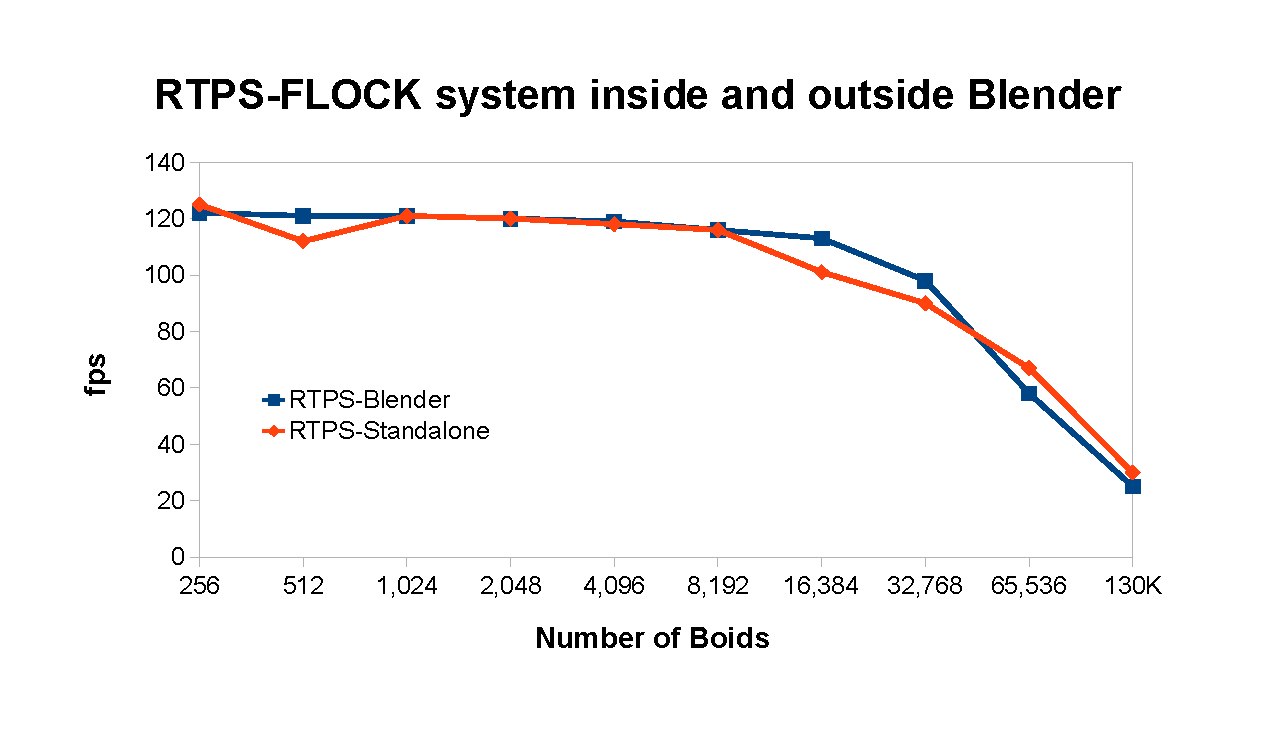
\includegraphics[scale=0.7]{figures/RTPSvsRTPS.pdf}
\caption{Timings of RTPS-FLOCK system: FLOCK system run from the standalone (outside the Blender Game Engine and the FLOCK system run from inside the Blender Game Engine}
\label{RTPSvsRTPS}
\end{center}
\end{figure}

% comments about the RTPS vs Blender plot
We also, measure the time that takes our Boids system and the time that Blender Boids system (outside the game engine) takes to run the same amount of particles with the same conditions stated above. Figure~\ref{RTPSvsBlender} shows the timings of the RTPS Boids system (computed in real-time) versus the Blender Boid system (outside the game engine, and only available for animations and simulations). The RTPS-FLOCK system has better performance than the Blender-Boids system all the time. Our FLOCK system renders up to almost $130K$ boids at the acceptable fps rate. Blender-Boids system renders up tp $8K$ boids at the acceptable fps.

%RTPS vs Blender
\begin{figure}[htbp]
\begin{center}
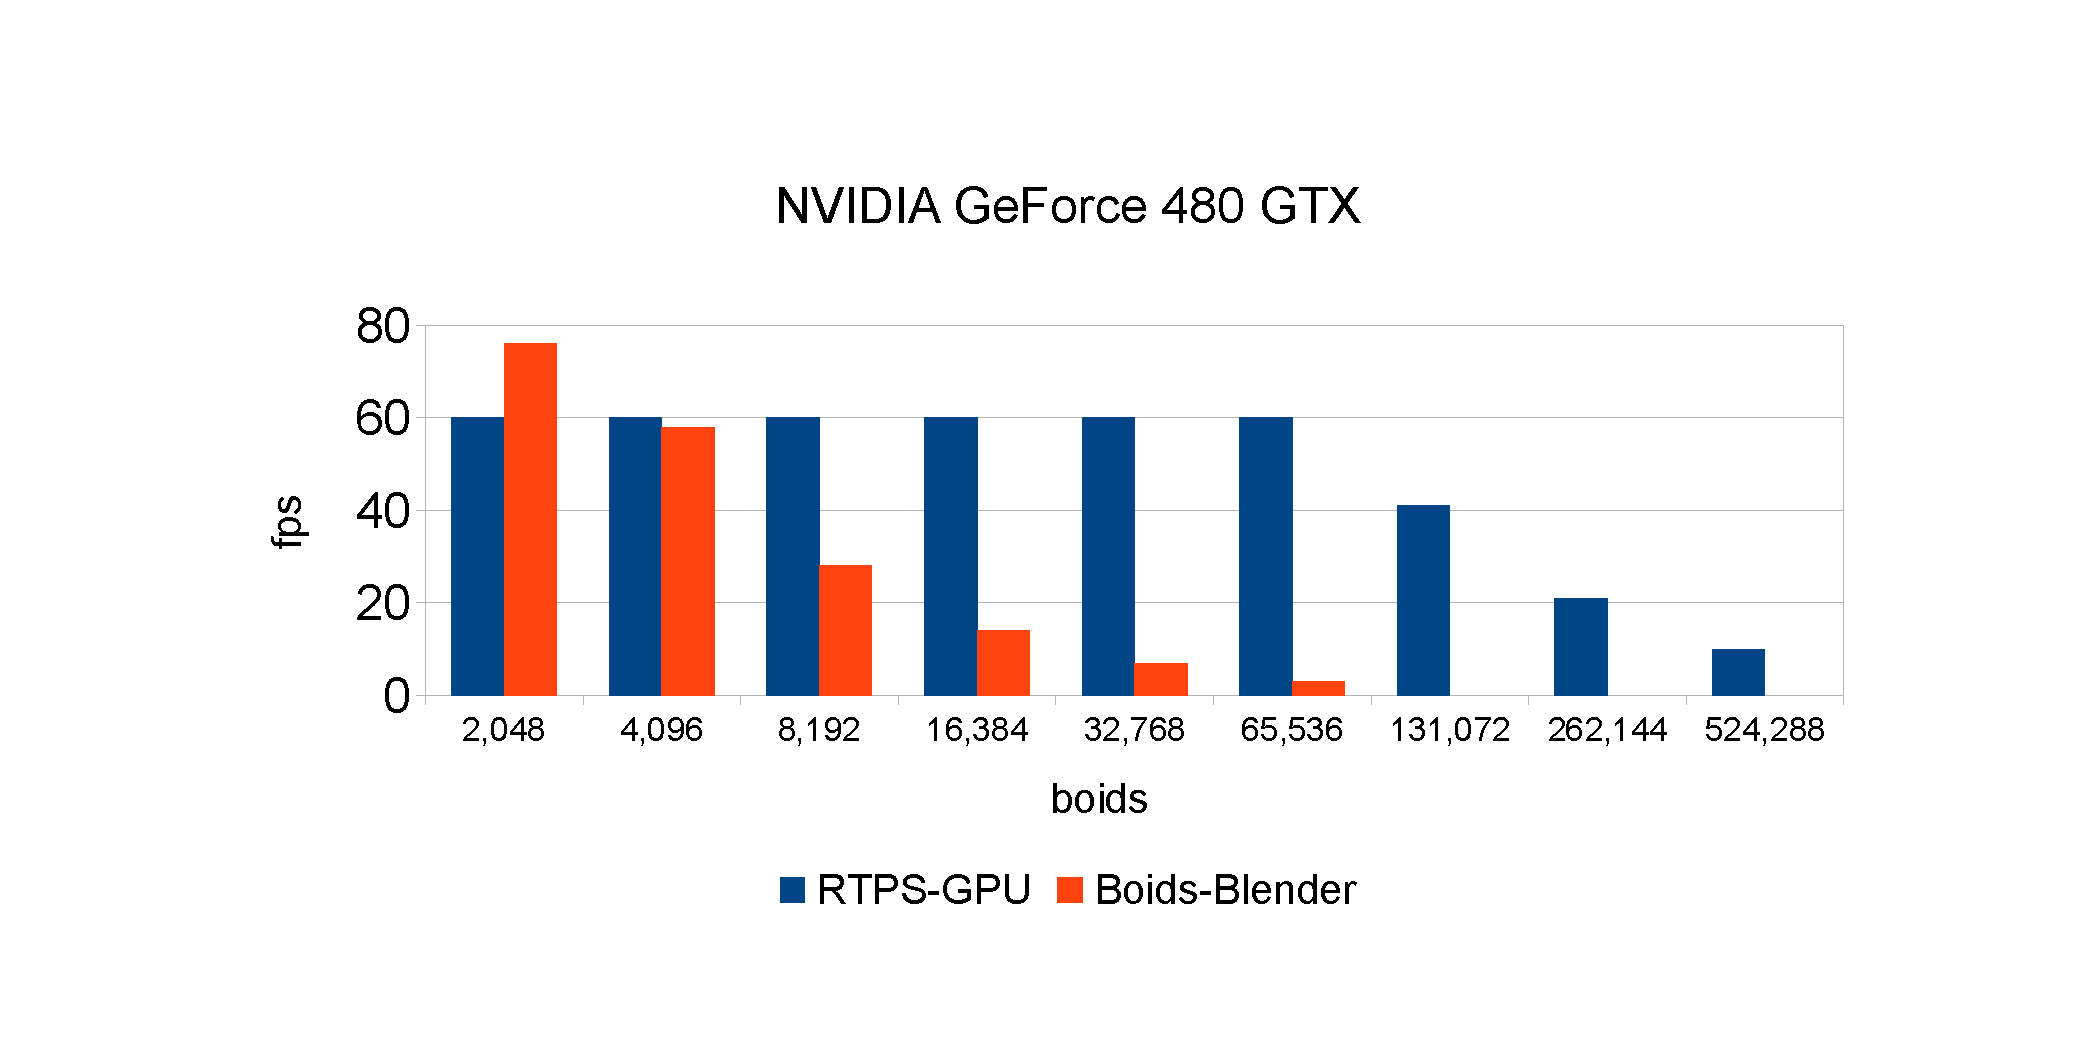
\includegraphics[scale=0.7]{figures/benchmarks.pdf}
\caption{Timings of the RTPS modifier and the Blender Boids system: the RTPS-GPU implementation outperforms the Blender Boids system}
\label{RTPSvsBlender}
\end{center}
\end{figure}

% comments about the speedup plot
The speedup of the RTPS-FLOCK system over the Blender Boids system is seen in Figure~\ref{speedup}. RTPS-FLOCK system is 20x faster than Blender-Boids system for flocks of $65K$. The frame rate of Blender-Boids system for flocks with more than $65K$ boids is less than a frame per second.

% speedup 
\begin{figure}[htbp]
\begin{center}
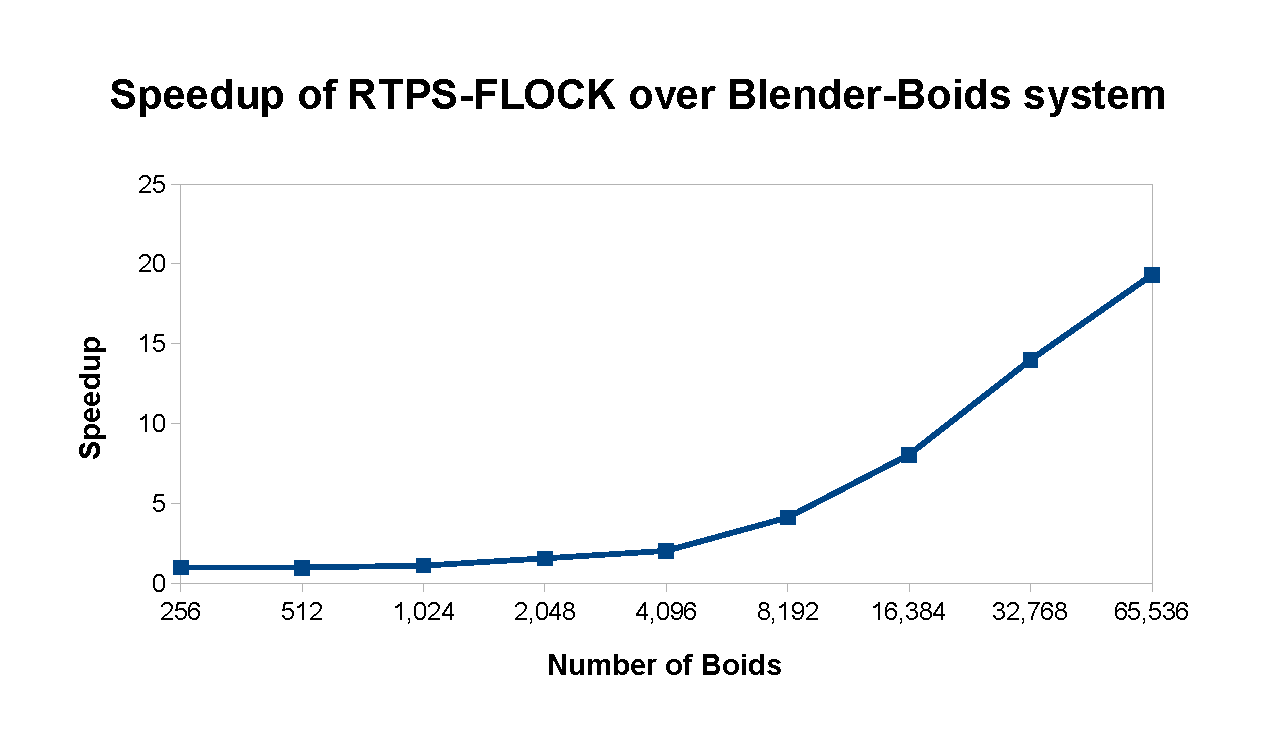
\includegraphics[scale=0.7]{figures/speedup.pdf}
\caption{Speedup of the FLOCK system of the RTPS library over the Blender Boids system}
\label{speedup}
\end{center}
\end{figure}

Comparing our performance with some of the benchmarks that were mentioned in Section~\ref{flockingGPU}, our flocking implementation still having better performance than them. The library BehaveRT was used to run autonomous characters simulations in real-time and visualization, in that paper Era et al. ran $130K$ boids at 15 fps, we ran $130K$ boids at 25 fps. The GPU computing device they used was a NVIDIA 8800GTS with 512 MB RAM while we used a NVIDIA 480GTX with 1.5 GB RAM. 

% comments about the timings per kernels
We also measured the inner performance of our FLOCK system. Timings of the execution of the kernels were measured. This timings were of a system with the settings specified above. The searching radius was constant trough out the benchmarks. Figure~\ref{kernelBench} shows that most of the kernels took the same amount of time for the different flock sizes. The only kernel that increased the time spent to be computed was the Rules kernel. This increase in time was because our searching radius was constant, therefore more boids are going to be used to compute the rules.

% benchmarks per kernels 
\begin{figure}[htbp]
\begin{center}
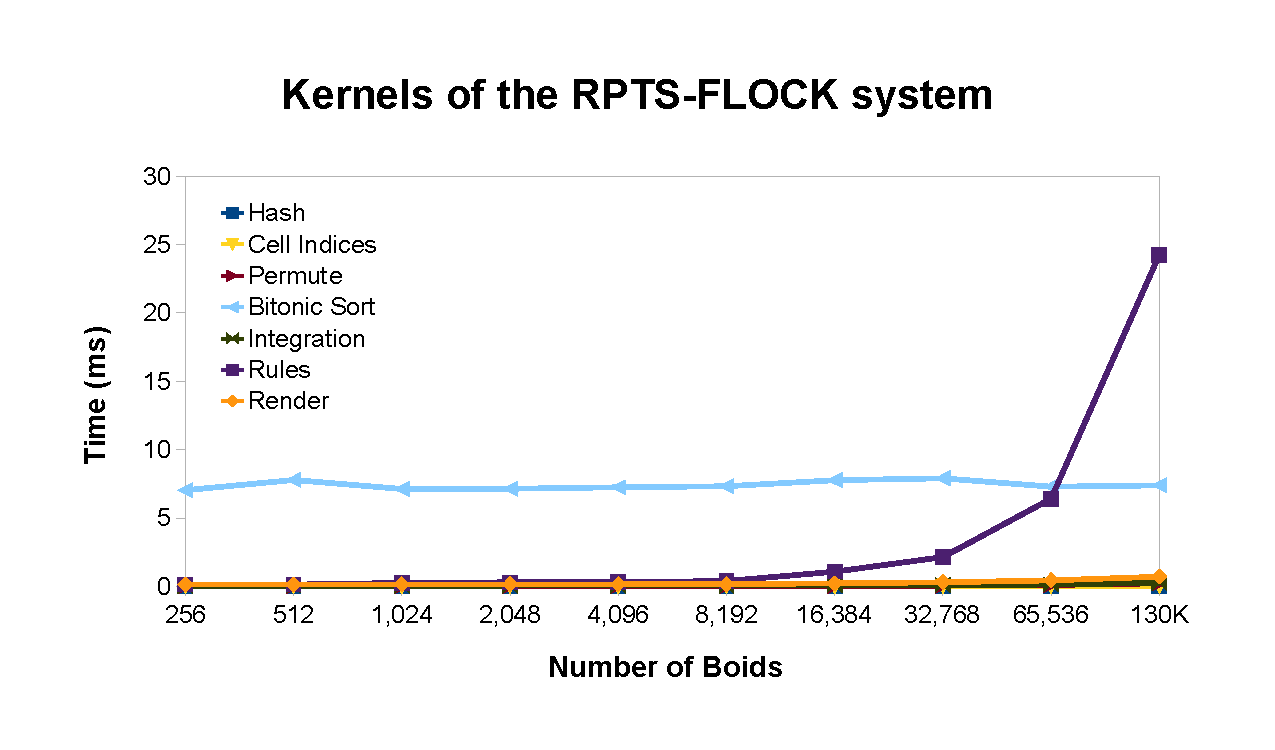
\includegraphics[scale=0.7]{figures/kernelsPlot.pdf}
\caption{Timings for the kernels executed by the FLOCK system of RTPS}
\label{kernelBench}
\end{center}
\end{figure}


% demos
\section{Demos}

\subsection{Symmetry of the Main Rules}
As discussed before the three main rules of flocking are: \textit{separation}, \textit{alignment}, and \textit{cohesion}. The velocity of each boid is determined by the linear combination of three effects, each one with its own weighing parameter. We seek to better understand the effect of each of these parameters. Consider first isolation each of the three effects: only a single effect is active at a time. 

The property of each term is best visualized with a an initial configuration of boids that is symmetric. To this end, we uniformly space the boids in a rectangular configuration.  From symmetry arguments, a boid in the top-left quadrant has the same relationship with respect to its neighbors as a boid in the same relative location in each of the other three quadrants. Thus the four-fold symmetry of the rectangle will be maintained during the time evolution of the boids. Figure~\ref{alignRule} shows the starting conditions of the boids. The symmetric moves of \textit{separation} and \textit{cohesion} are shown in Figures~\ref{sepRule} and~\ref{cohRule}, respectively. These figures show 144 boids in a centralized square inside a $5$x$5$x$5$ box.

The current available rendering methods in RTPS does not let us present a visual demo od the symmetry of alignment. Although \textit{alignment} is also symmetric. Consider starting with the same initial conditions than in Figure~\ref{alignRule}, what only matters for \textit{alignment} is the velocities. If the boids have identical velocities (in magnitude and directions) initially, they will continue in the same direction. Recalling that we only want to prove that the rules are symmetric assuming that they start from a symmetric configuration, and we assure that the symmetry is preserved.

% alignment
\begin{figure}[htbp]
\begin{center}
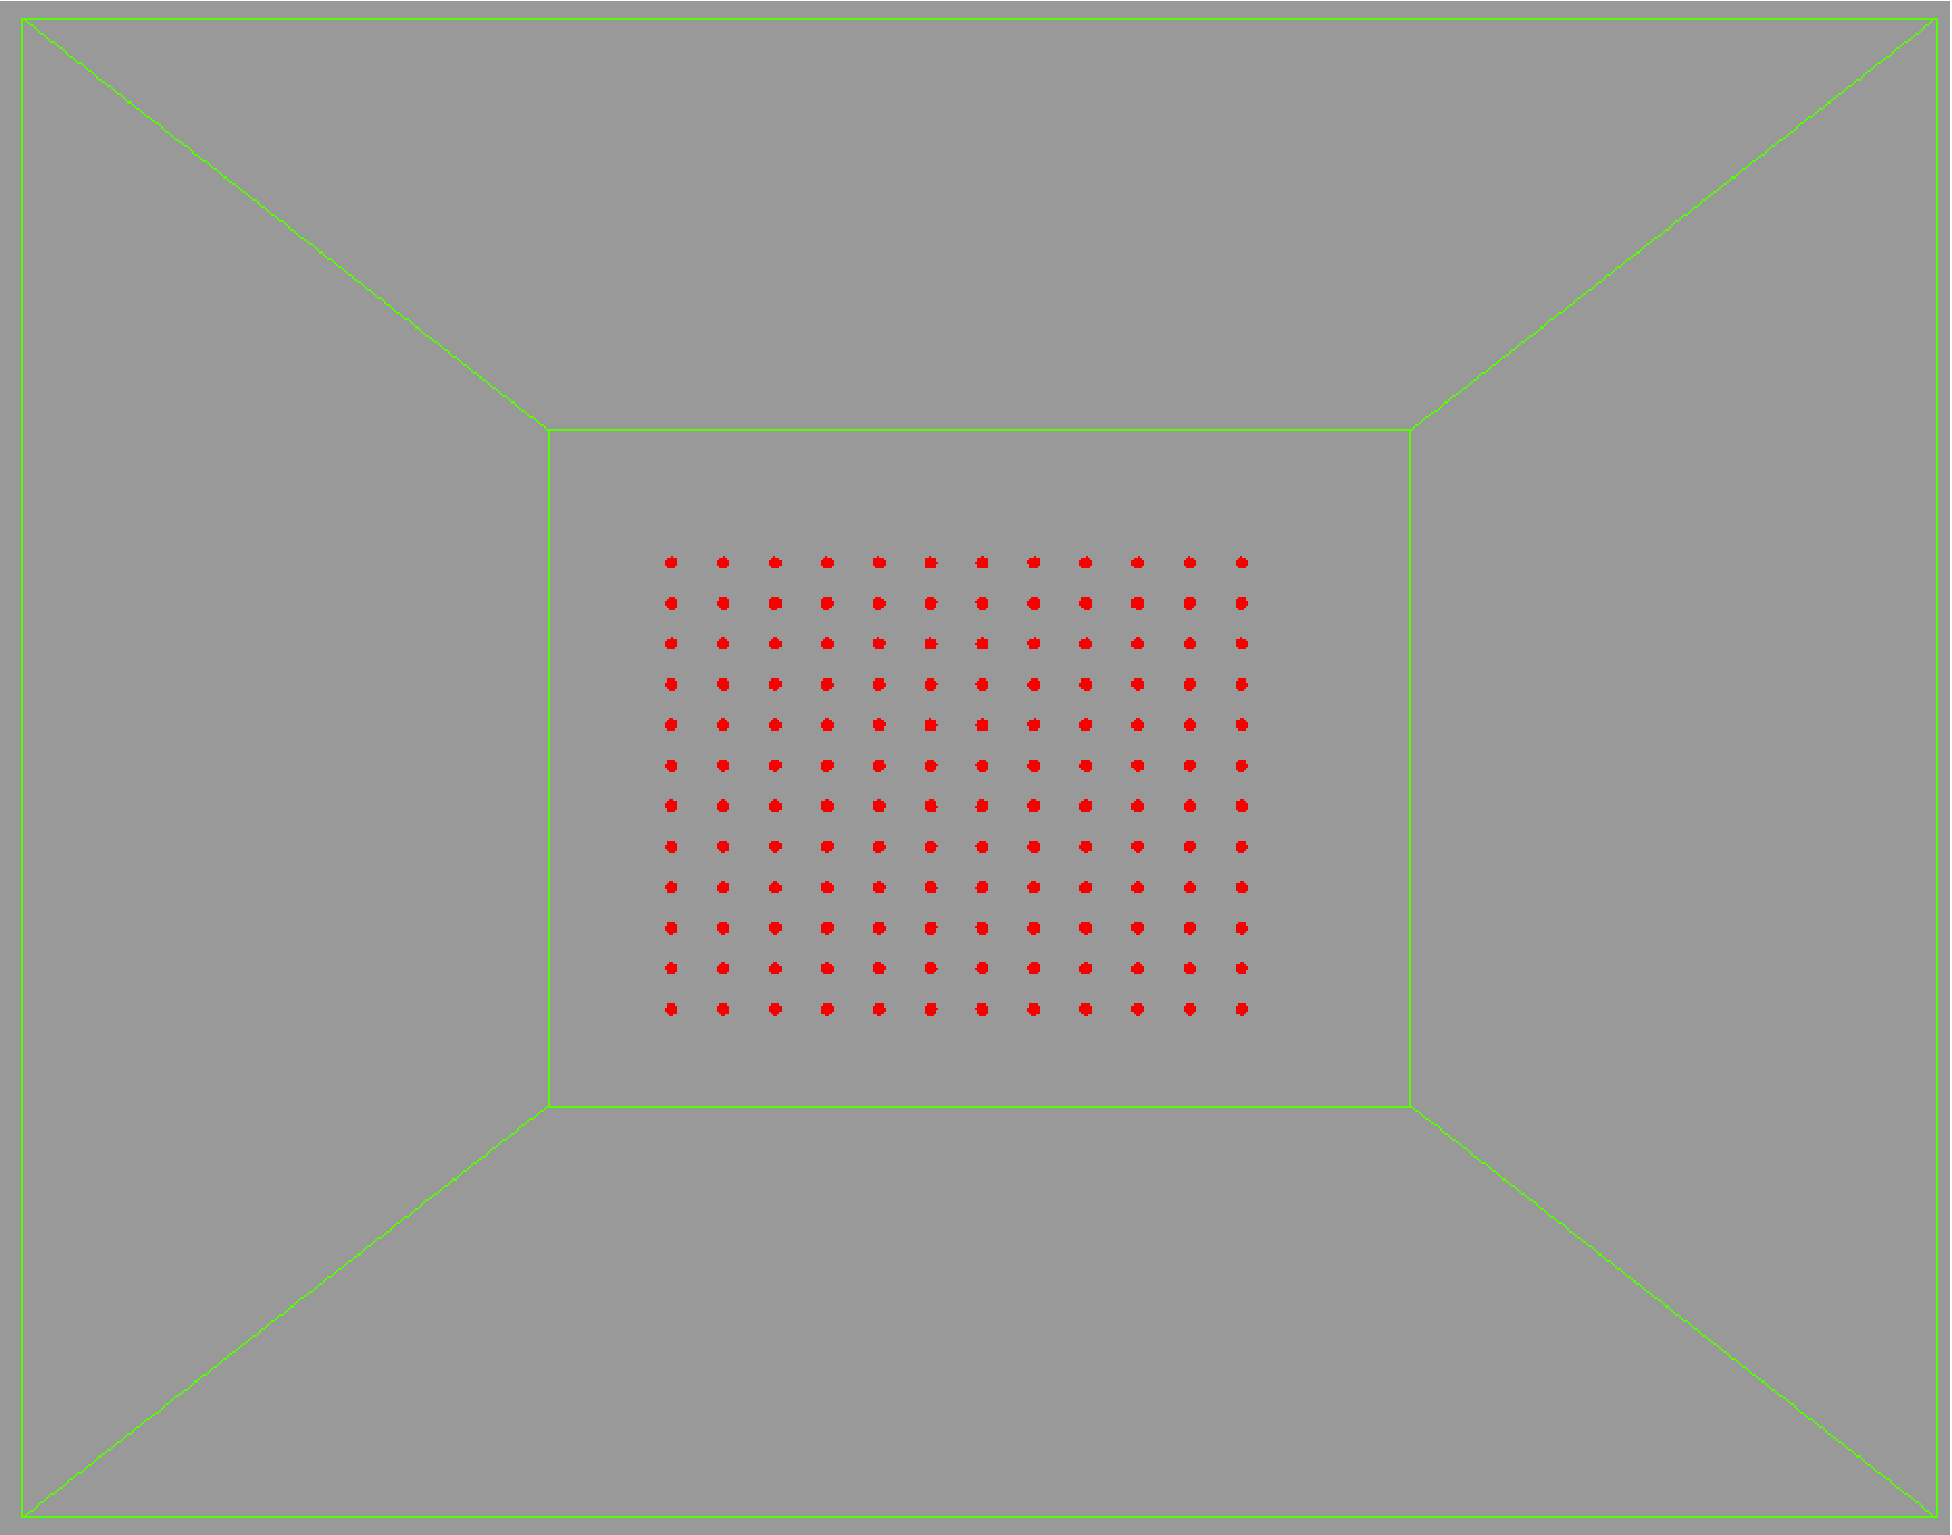
\includegraphics[scale=0.5]{figures/align.pdf}
\caption{Initial state of the boids: the weights for each of the rules are zero, the boids are initialized equally spaced forming a symmetric square}
\label{alignRule}
\end{center}
\end{figure}

% separation
\begin{figure}[htbp]
\begin{center}$
\begin{array}{cc}
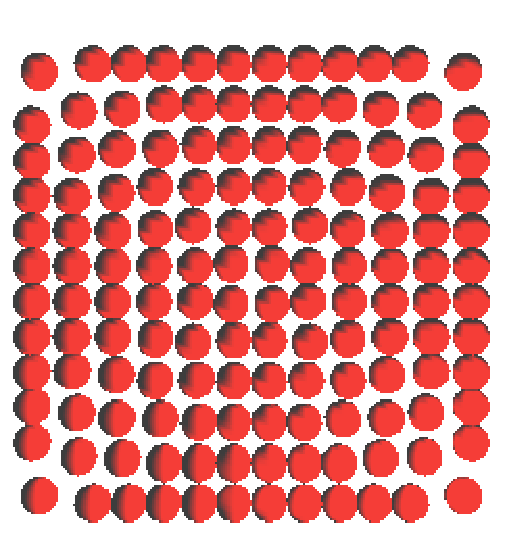
\includegraphics[scale= 0.5]{figures/sep1.pdf} &
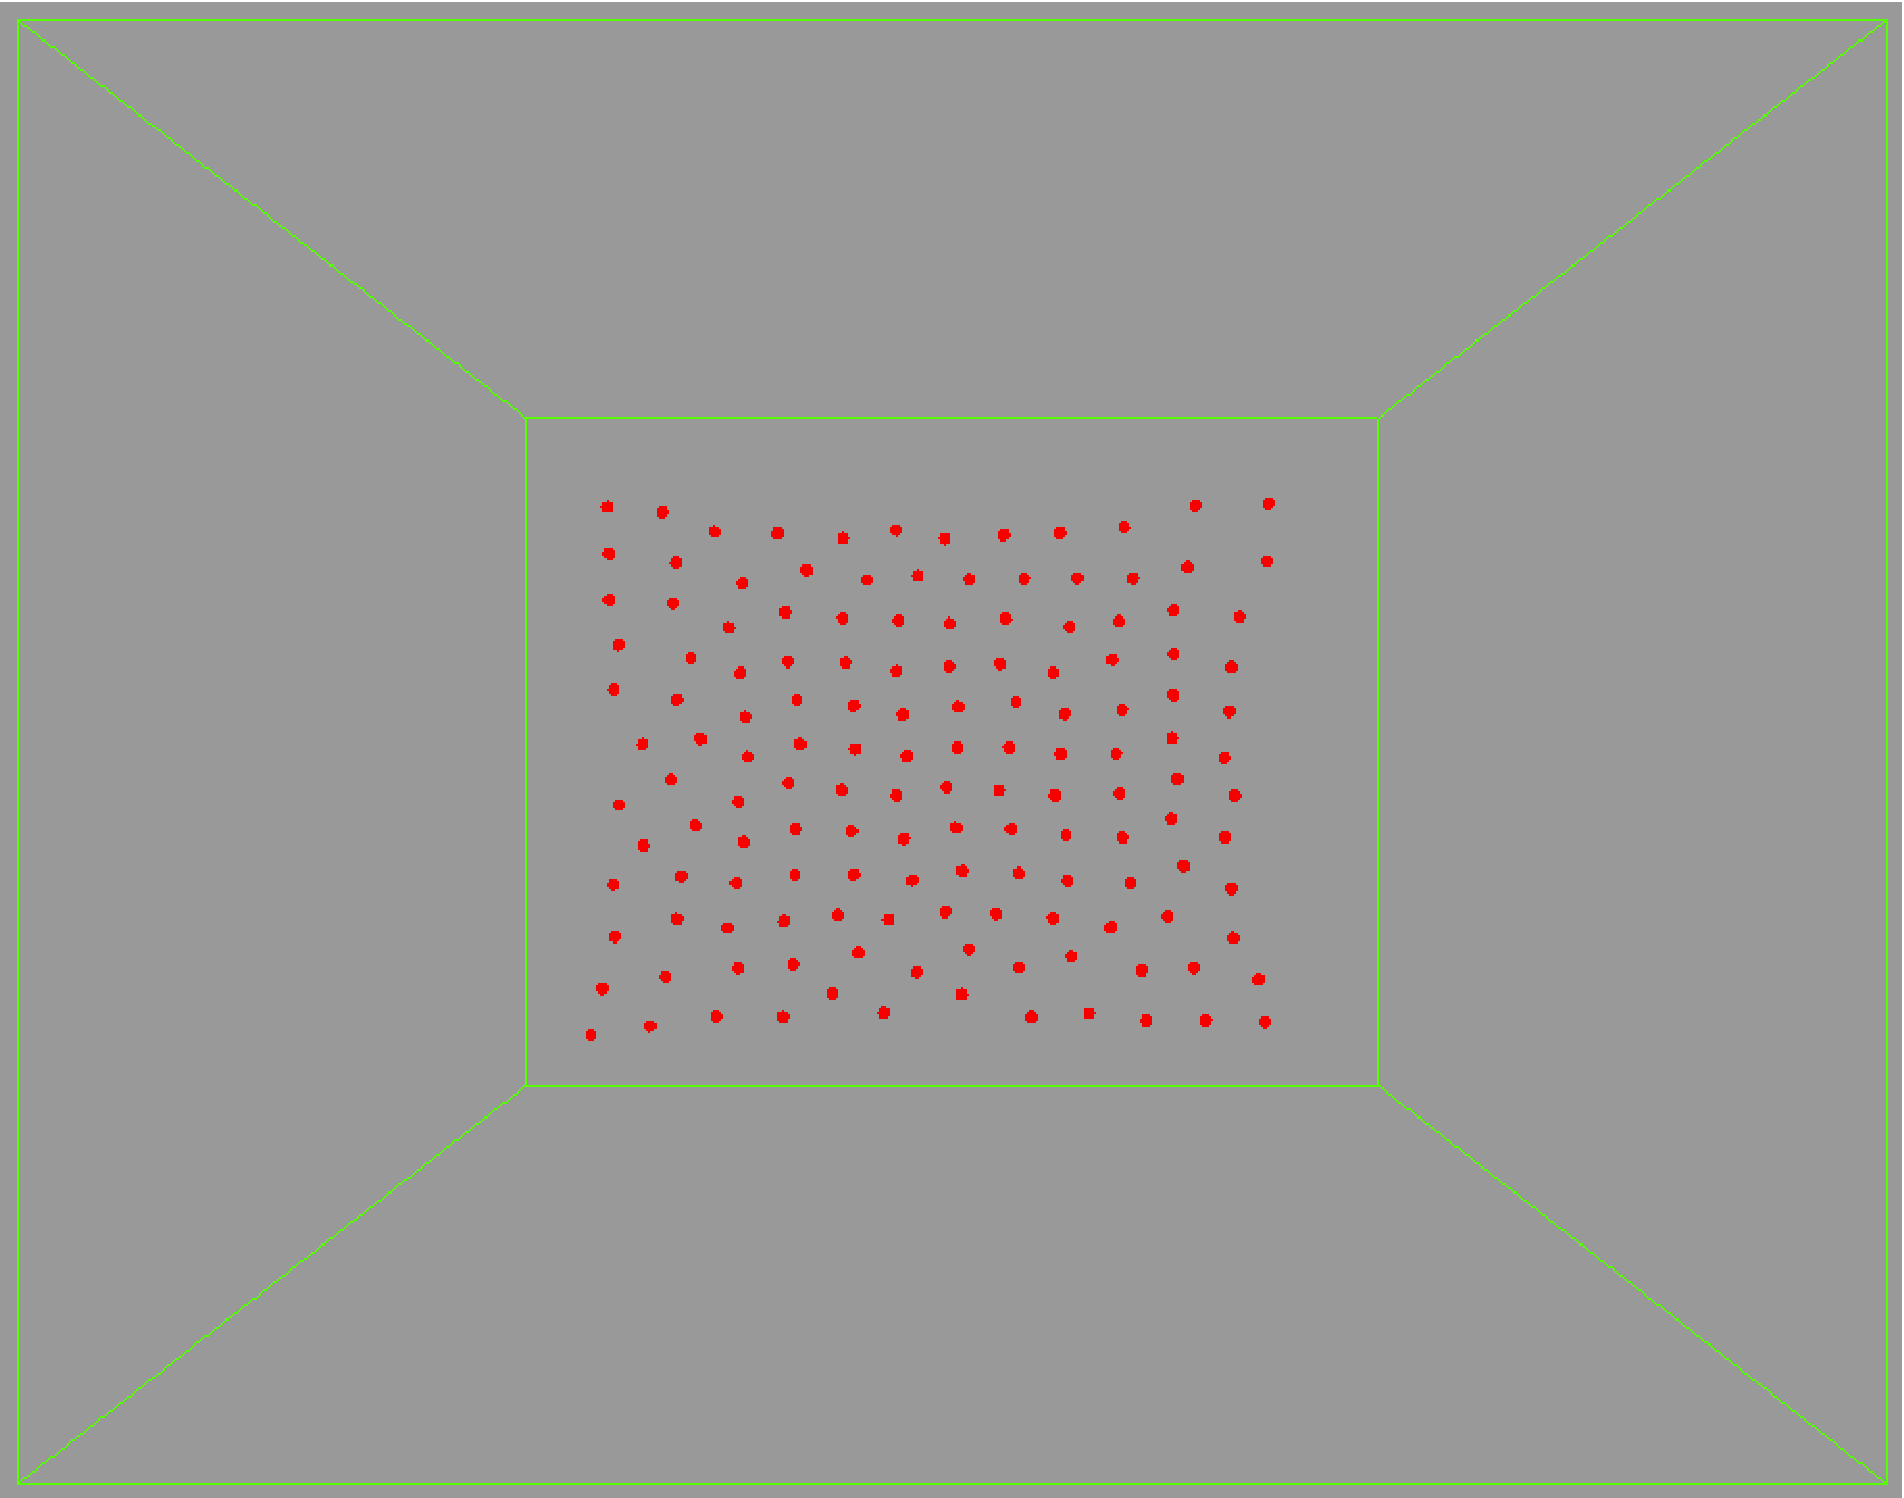
\includegraphics[scale= 0.5]{figures/sep2.pdf}
\end{array}$
\end{center}
\caption{Screenshots of the separation rule: the weight for \textit{separation} was set to 1 while the weights of the other two rules were set to zero, the boids started to spread out symmetrically}
\label{sepRule}
\end{figure}

% cohesion
\begin{figure}[htbp]
\begin{center}
\begin{tabular}{cc}
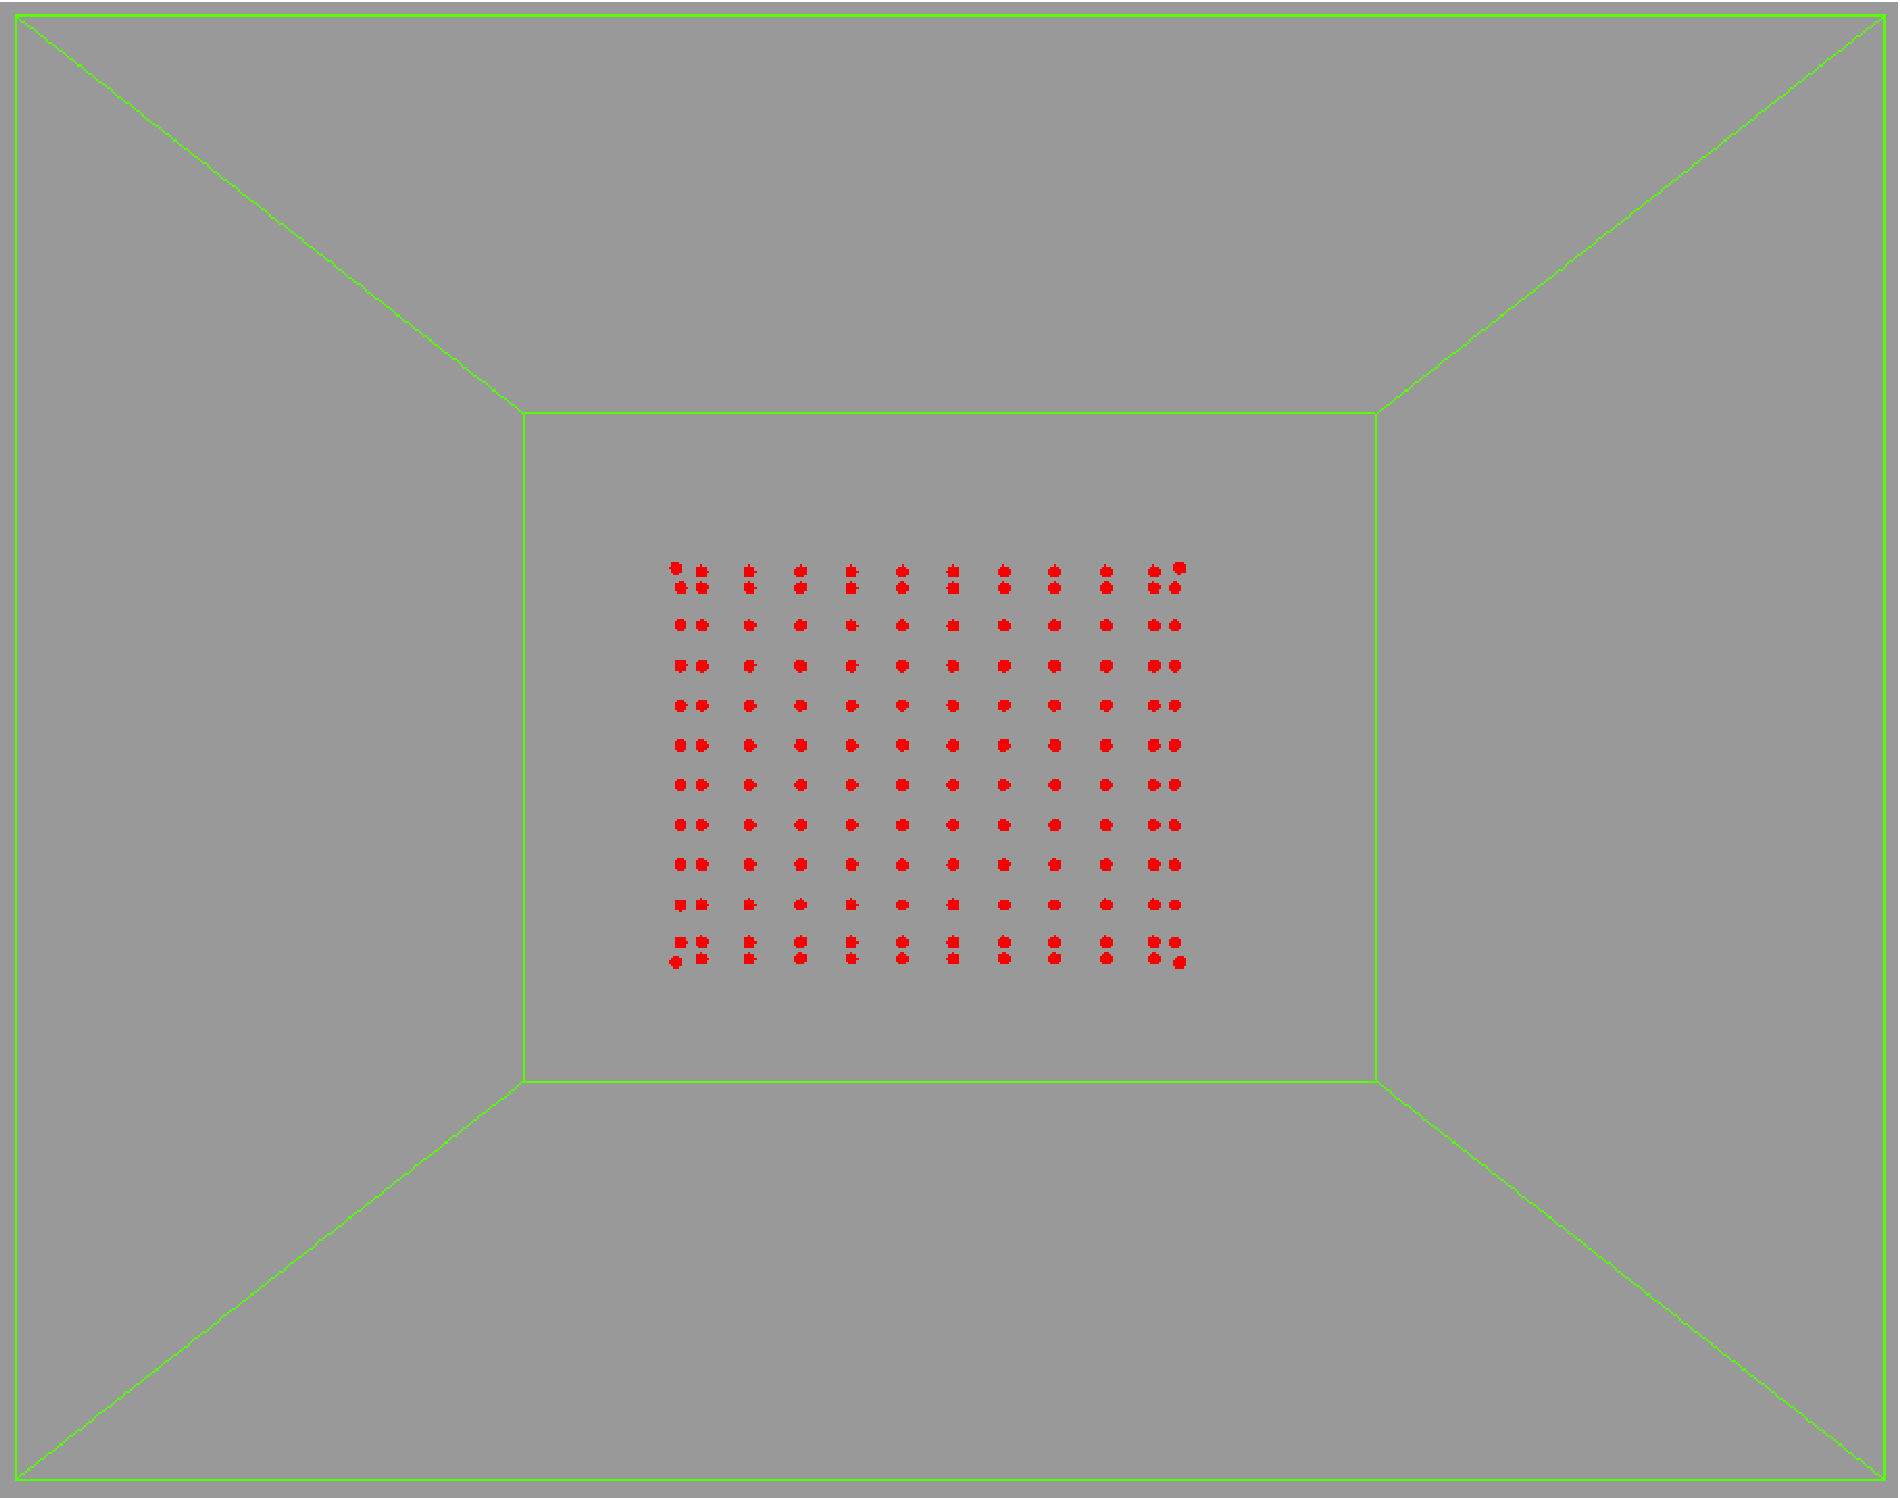
\includegraphics[scale= 0.5]{figures/coh1.pdf} &
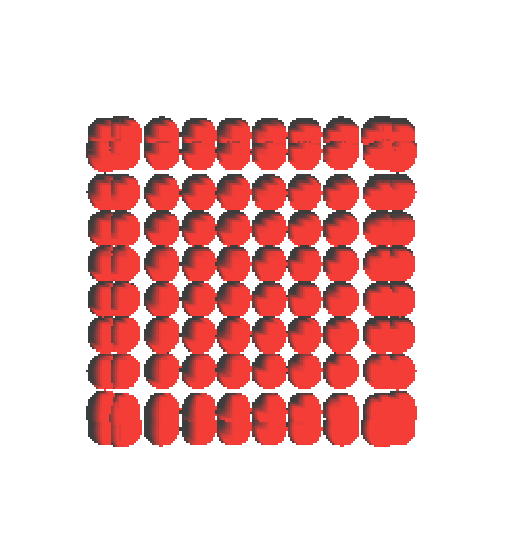
\includegraphics[scale= 0.5]{figures/coh2.pdf} \\

\includegraphics[scale= 0.5]{figures/coh3.pdf} &
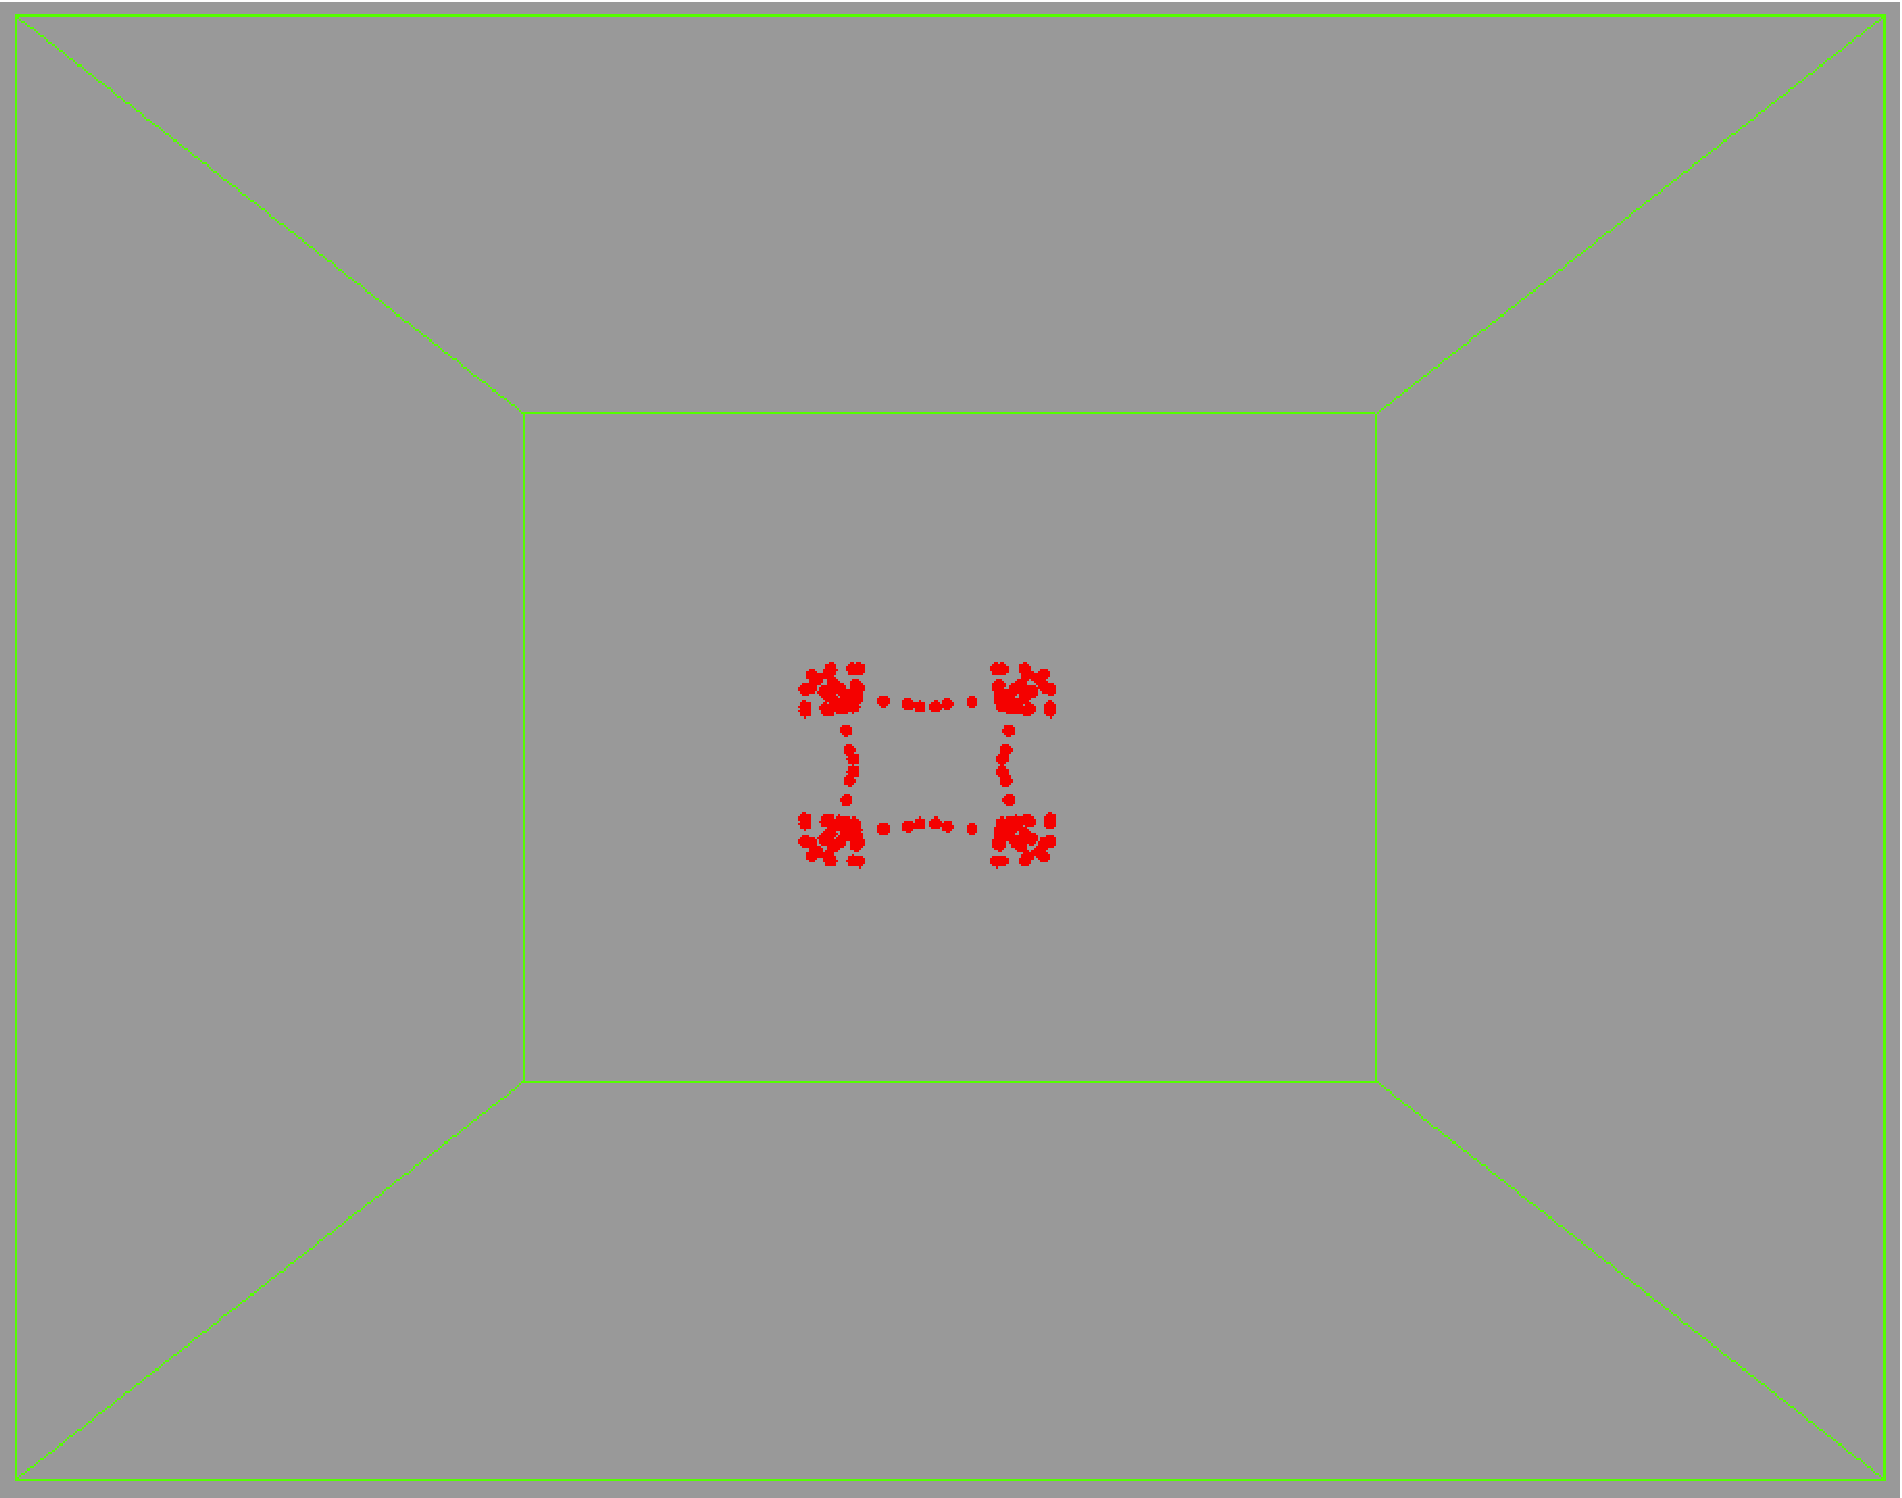
\includegraphics[scale= 0.5]{figures/coh4.pdf}
\end{tabular}
\end{center}
\caption{Screenshots of the cohesion rule: the weight for the \textit{cohesion} rule was set to 1 while the weights for the other two rules were set to zero, the boids move towards the center causing them to merge symmetrically}
\label{cohRule}
\end{figure}

% Goal demo
\subsection{Goal Demo}
The \textit{goal} and \textit{avoid} rules currently are available to be used only in the RTPS standalone code. They have not beed added to the RTPS modifier yet. 

In this demo we simulate a swarm of bees, when they try to approach the target (in the demo a blue box) which is their hive. The center of the cube is used as the coordinates of the target. The number of boids emitted is 648. Only the goal rules is computed, with a weight constant of 1. The settings of this demo were a maximum speed equals to 2, and a searching radius of 1.5. 

\begin{figure}[htbp]
\begin{center}$
\begin{array}{ccc}
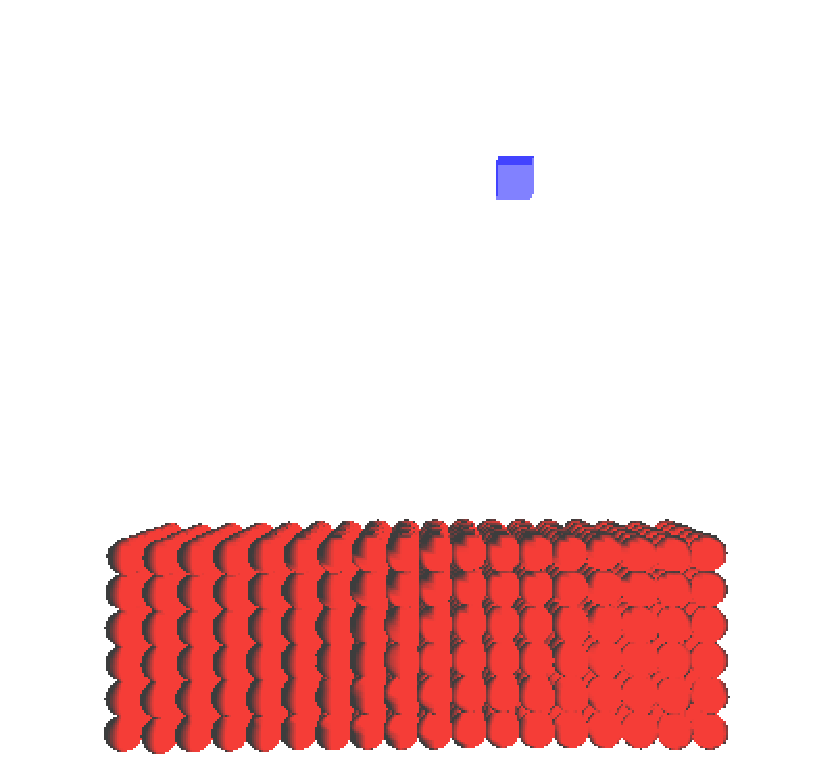
\includegraphics[scale=0.35]{figures/demo_goal1.pdf} &&
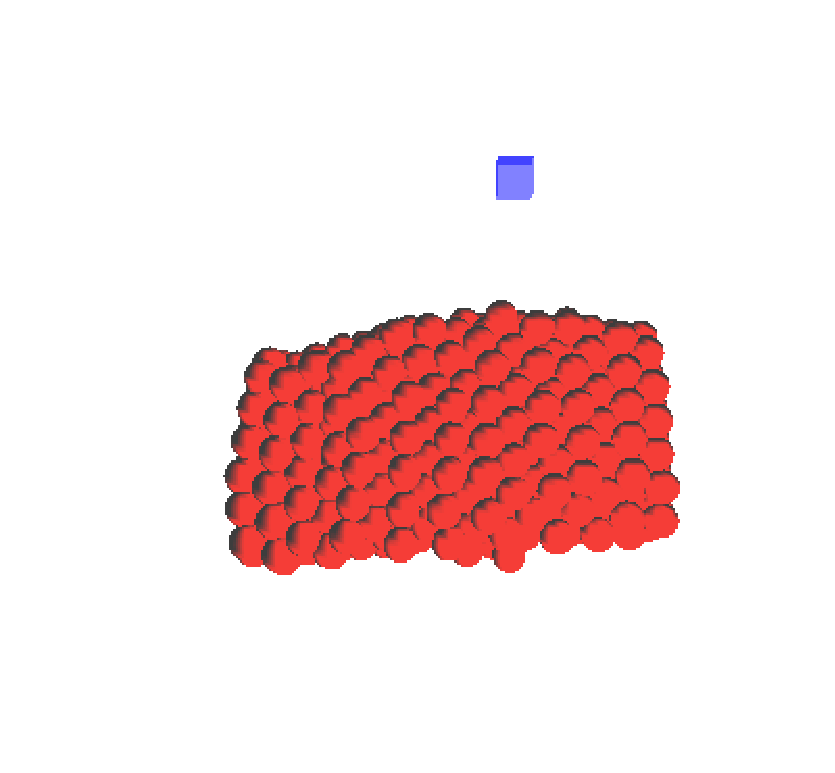
\includegraphics[scale=0.35]{figures/demo_goal2.pdf} \\ \\
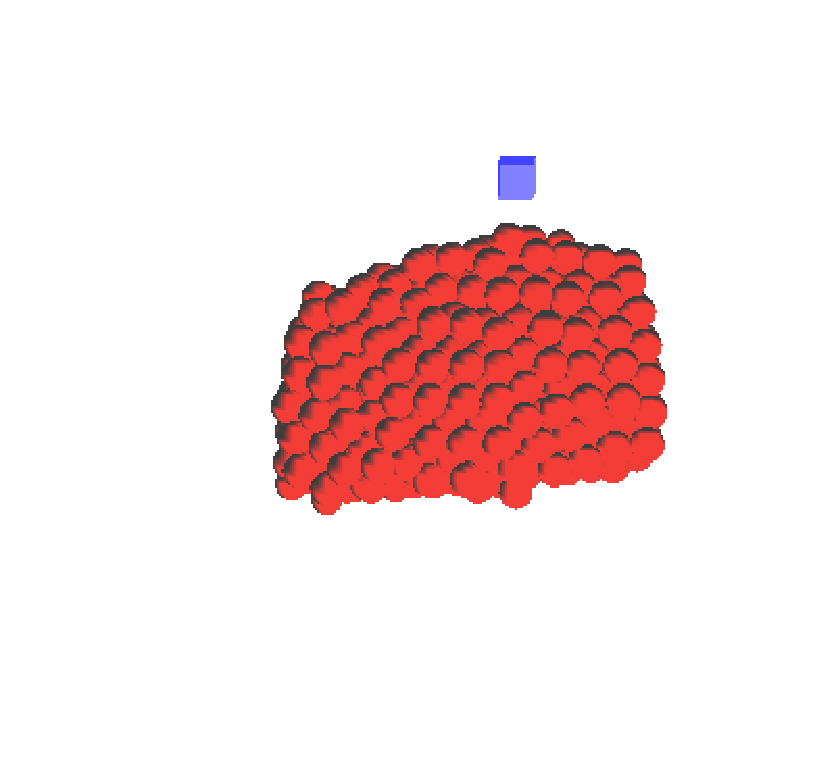
\includegraphics[scale=0.35]{figures/demo_goal3.pdf} &&
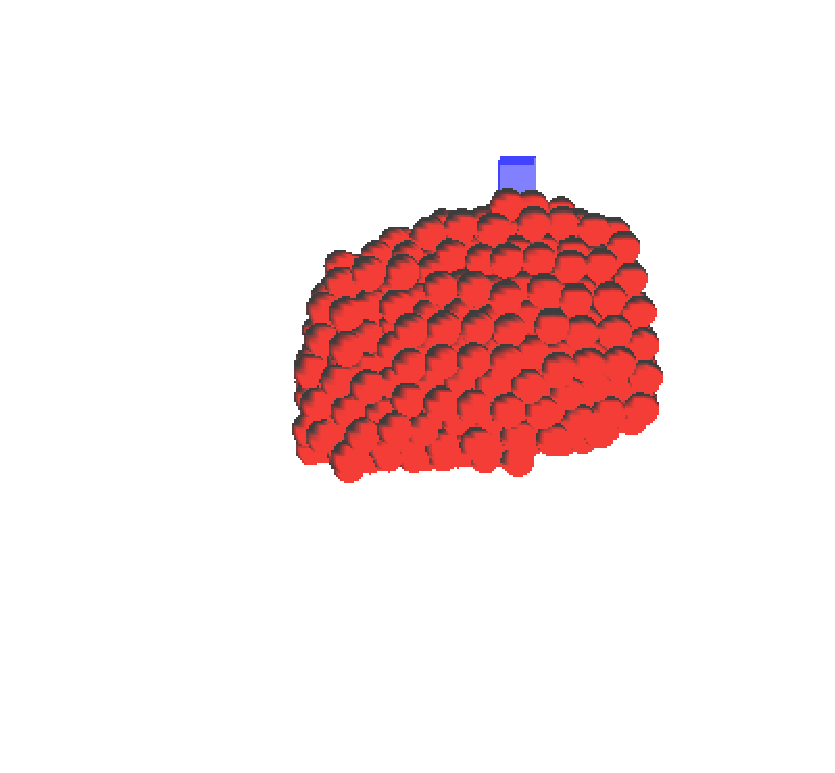
\includegraphics[scale=0.35]{figures/demo_goal4.pdf} \\ \\
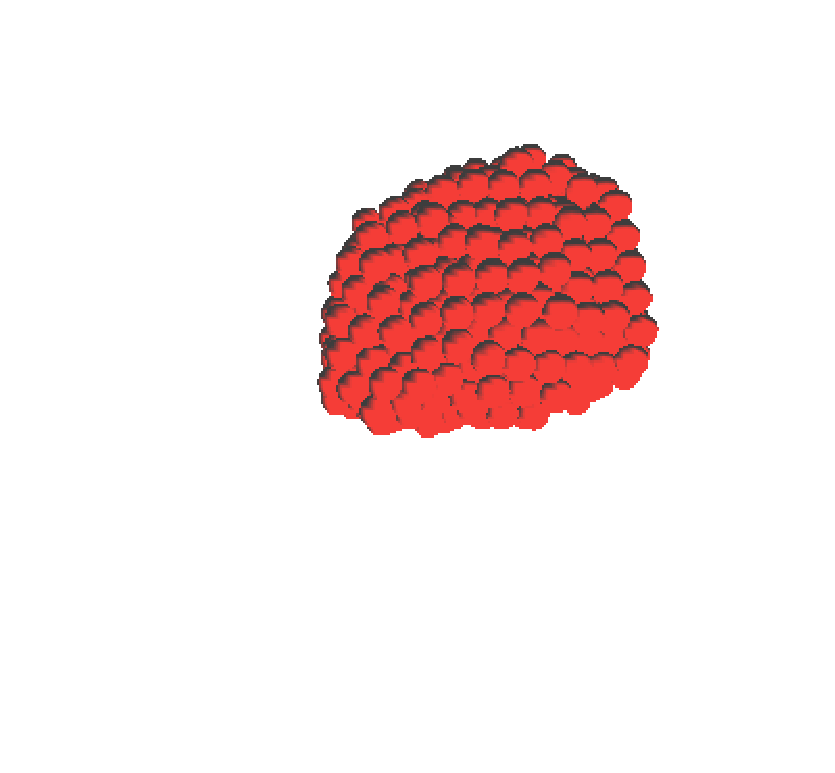
\includegraphics[scale=0.35]{figures/demo_goal5.pdf} &&
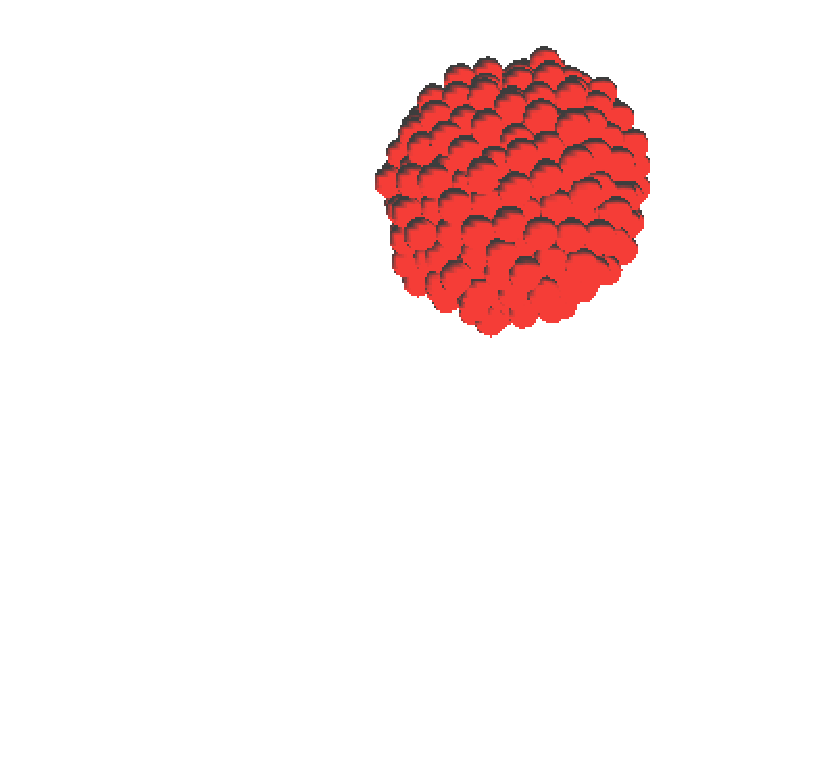
\includegraphics[scale=0.35]{figures/demo_goal6.pdf}
\end{array}$
\end{center}
\caption{Screenshots of the demonstration of the \textit{goal} rule: there are 648 boids and the blue cube is the target of the flock.}
\label{demo_goal}
\end{figure}
 
Figure~\ref{demo_goal} shows a series of screenshots of this demo. The flock starts from an artificial cube shape. They start approaching the target until they got it. After the boids found the target, they stay rounding it. 

We ran another demo in which the three main steering behaviors plus the \textit{goal} rule were used to compute the behavior of the boids. Figure~\ref{goal_4rules} shows the resulting flock. Each rule was weighted equally. A minimum separation distance of 2 and a searching radius of 2.5 were used. The initial positions of the boids were the same than in Figure~\ref{demo_goal}. From the Figure we can see that the boids are more separated than in the first example, this is because we are using the separation rule and the minimum separation distance is double than the initial distance that separates the boids. Although, four rules were computed we can see that the objective of the flock was made.

% 4 rules
\begin{figure}[htbp]
\begin{center}
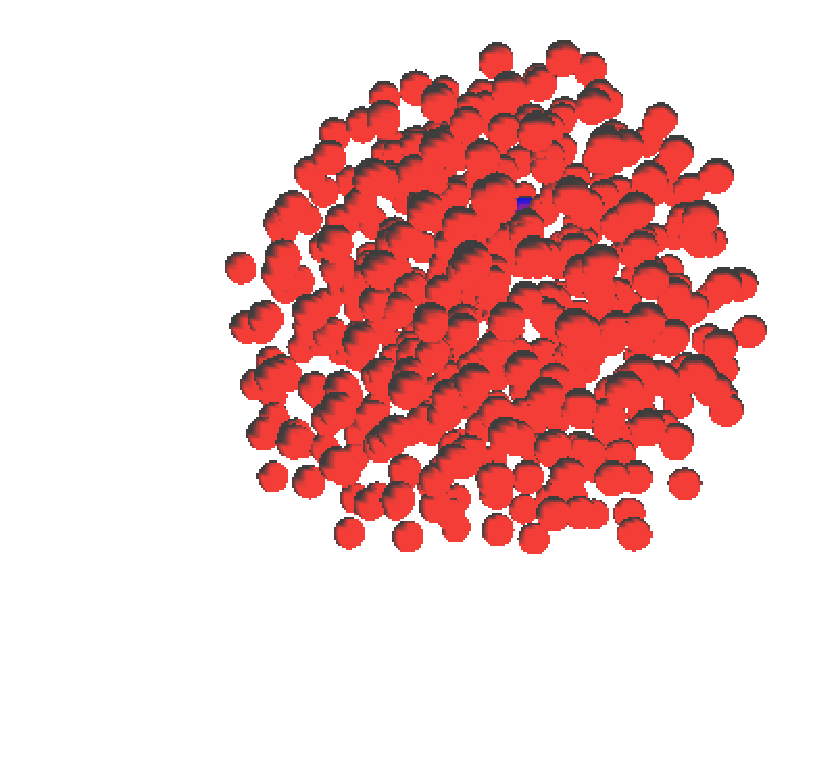
\includegraphics[scale=0.35]{figures/demo_goal_4rules.pdf}
\caption{Screenshot of the flock following the target: \textit{separation}, \textit{alignment}, \textit{cohesion}, and \textit{goal} rules were used to compute the behavior of the boids.}
\label{goal_4rules}
\end{center}
\end{figure}

% Blender demo
\subsection{Blender Demo}

The following Blender demo of the RTPS library uses one hose that emit 500 boids. This demo would simulate a crowd of people. Figure~\ref{crowd_prop} shows the properties to create the hose, and Figure~\ref{crowd_modifier} shows the settings used on this demo. 

\begin{figure}[htbp]
\begin{center}
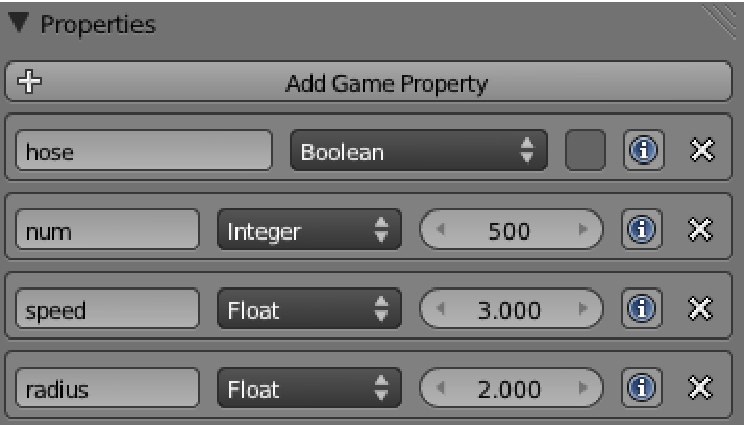
\includegraphics[scale=0.7]{figures/demo_crowds_prop.pdf}
\caption{Logic editor properties area showing the properties used to create the hose of the crowding simulation demo}
\label{crowd_prop}
\end{center}
\end{figure}

\begin{figure}[htbp]
\begin{center}
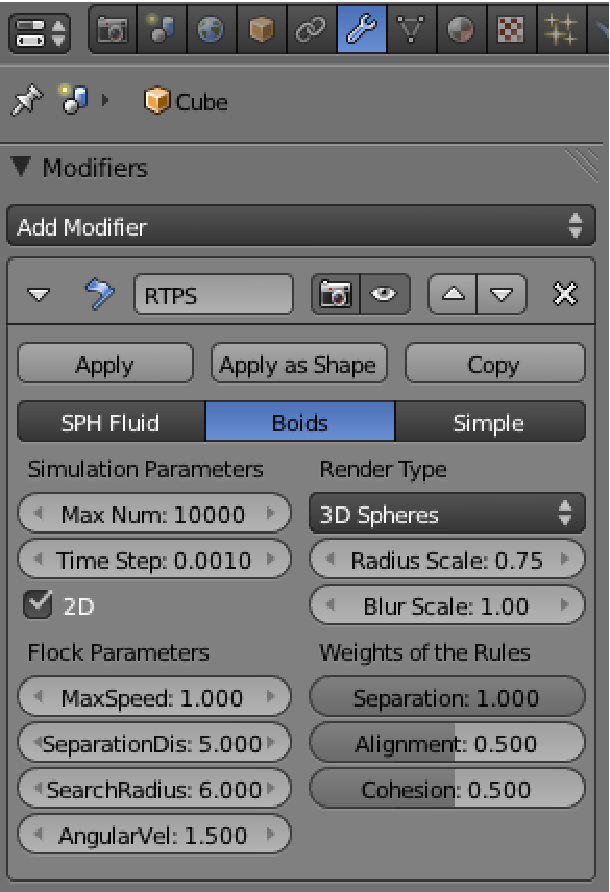
\includegraphics[scale=0.8]{figures/demo_crowds_modifier.pdf}
\caption{RTPS modifier showing the settings of the crowd simulation demo}
\label{crowd_modifier}
\end{center}
\end{figure}

Figure~\ref{crowd_shots} shows the screenshots of the demo. The emitter hose, starts emitting the boids at the center of the world. Then, the boids start reacting according to the settings of the simulation. Finally, the boids are spread out into the world domain and still following the rules.

\begin{figure}[htbp]
\begin{center}$
\begin{array}{c}
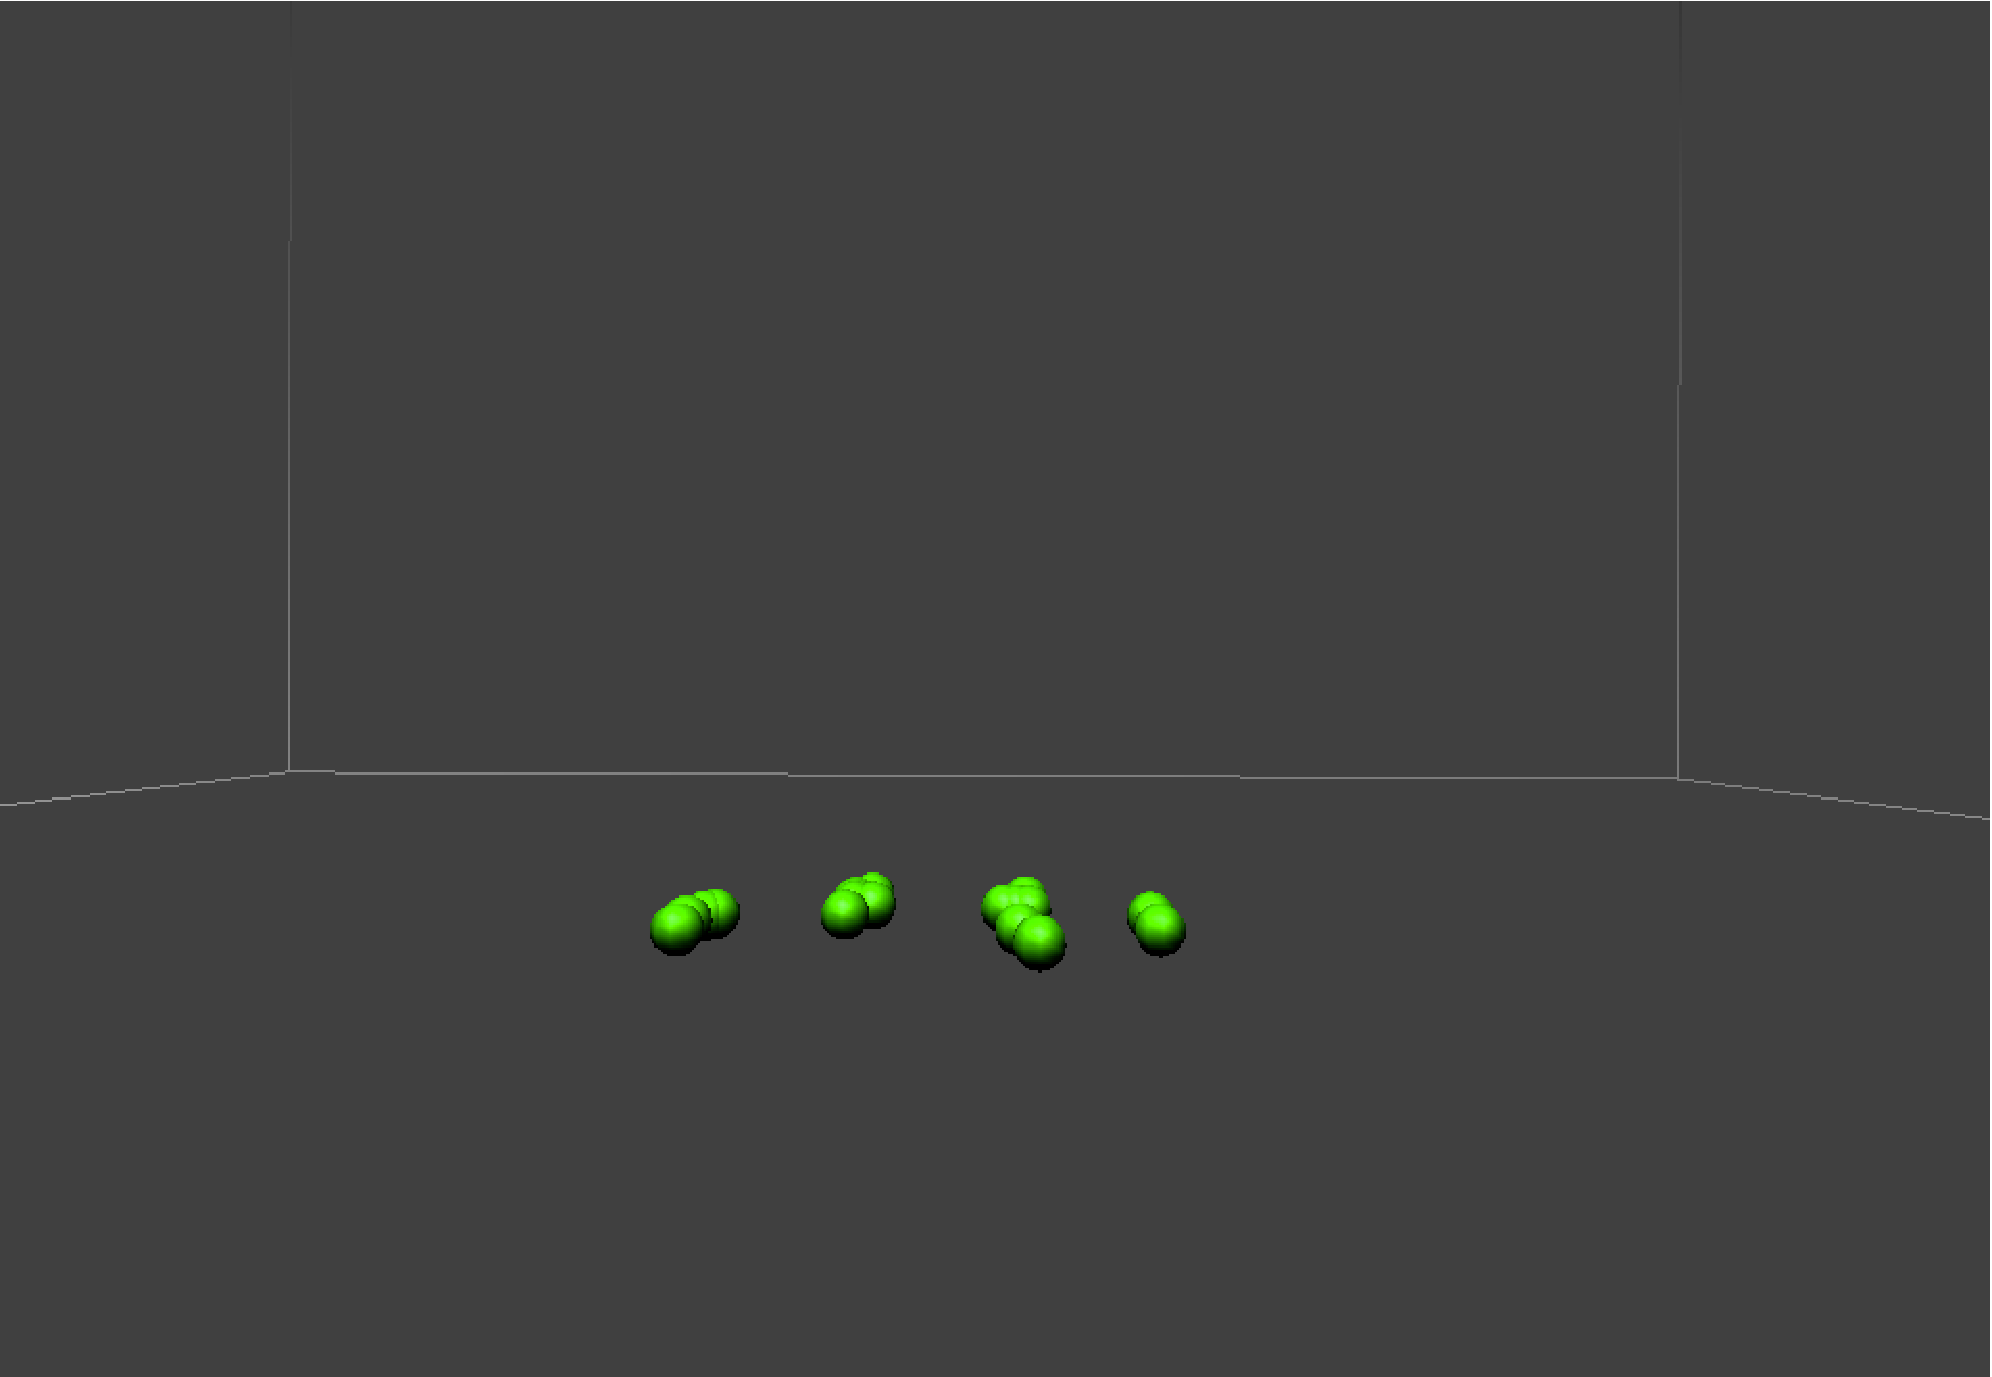
\includegraphics[scale=0.28]{figures/demo_crowds1.pdf} \\
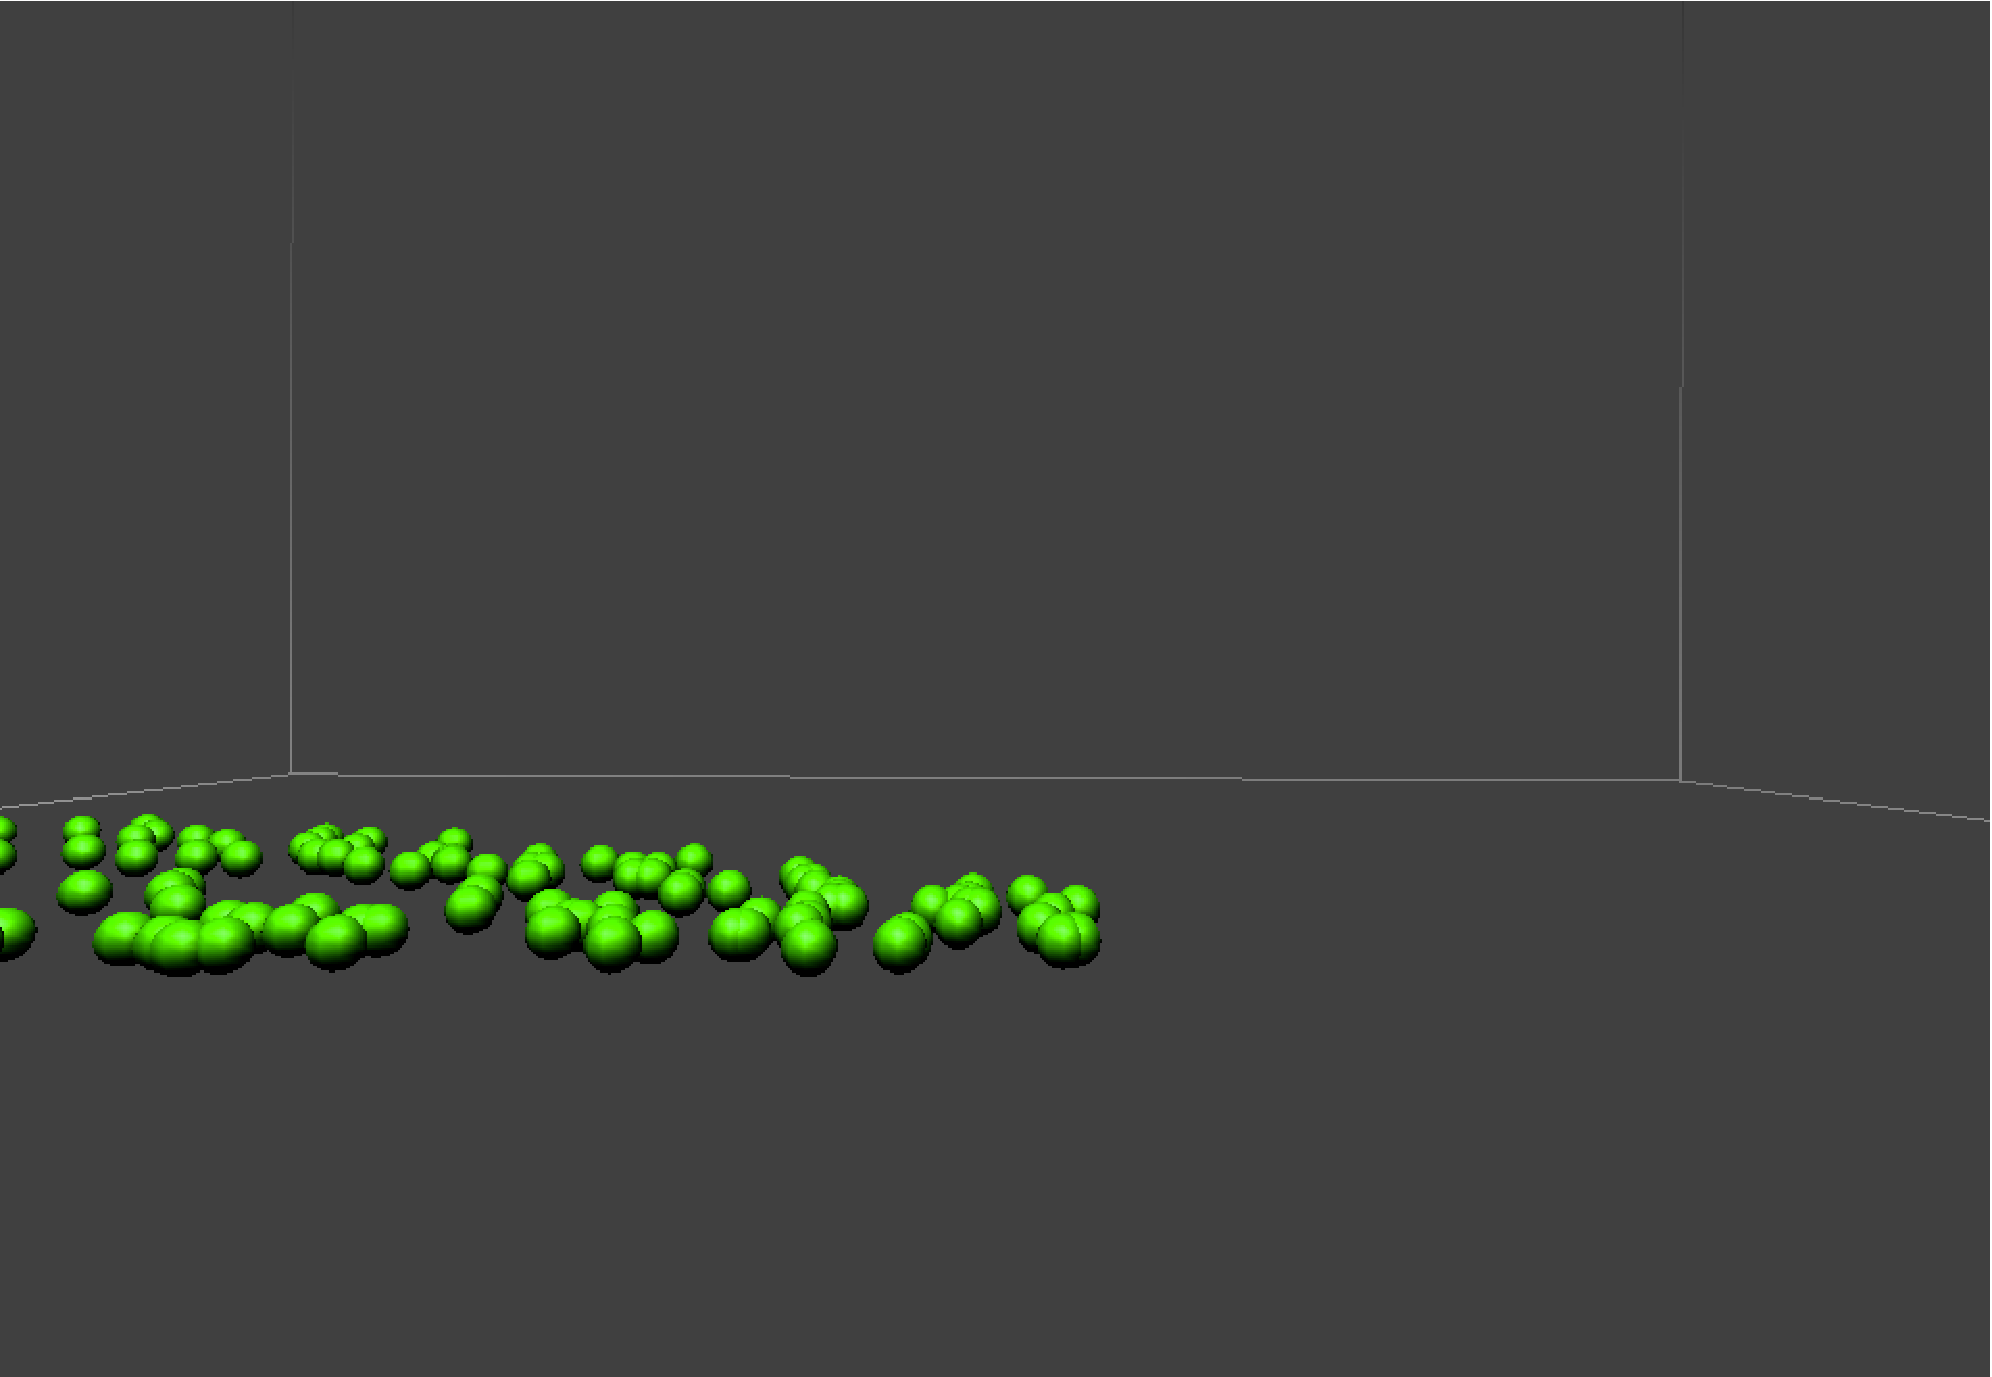
\includegraphics[scale=0.28]{figures/demo_crowds2.pdf} \\
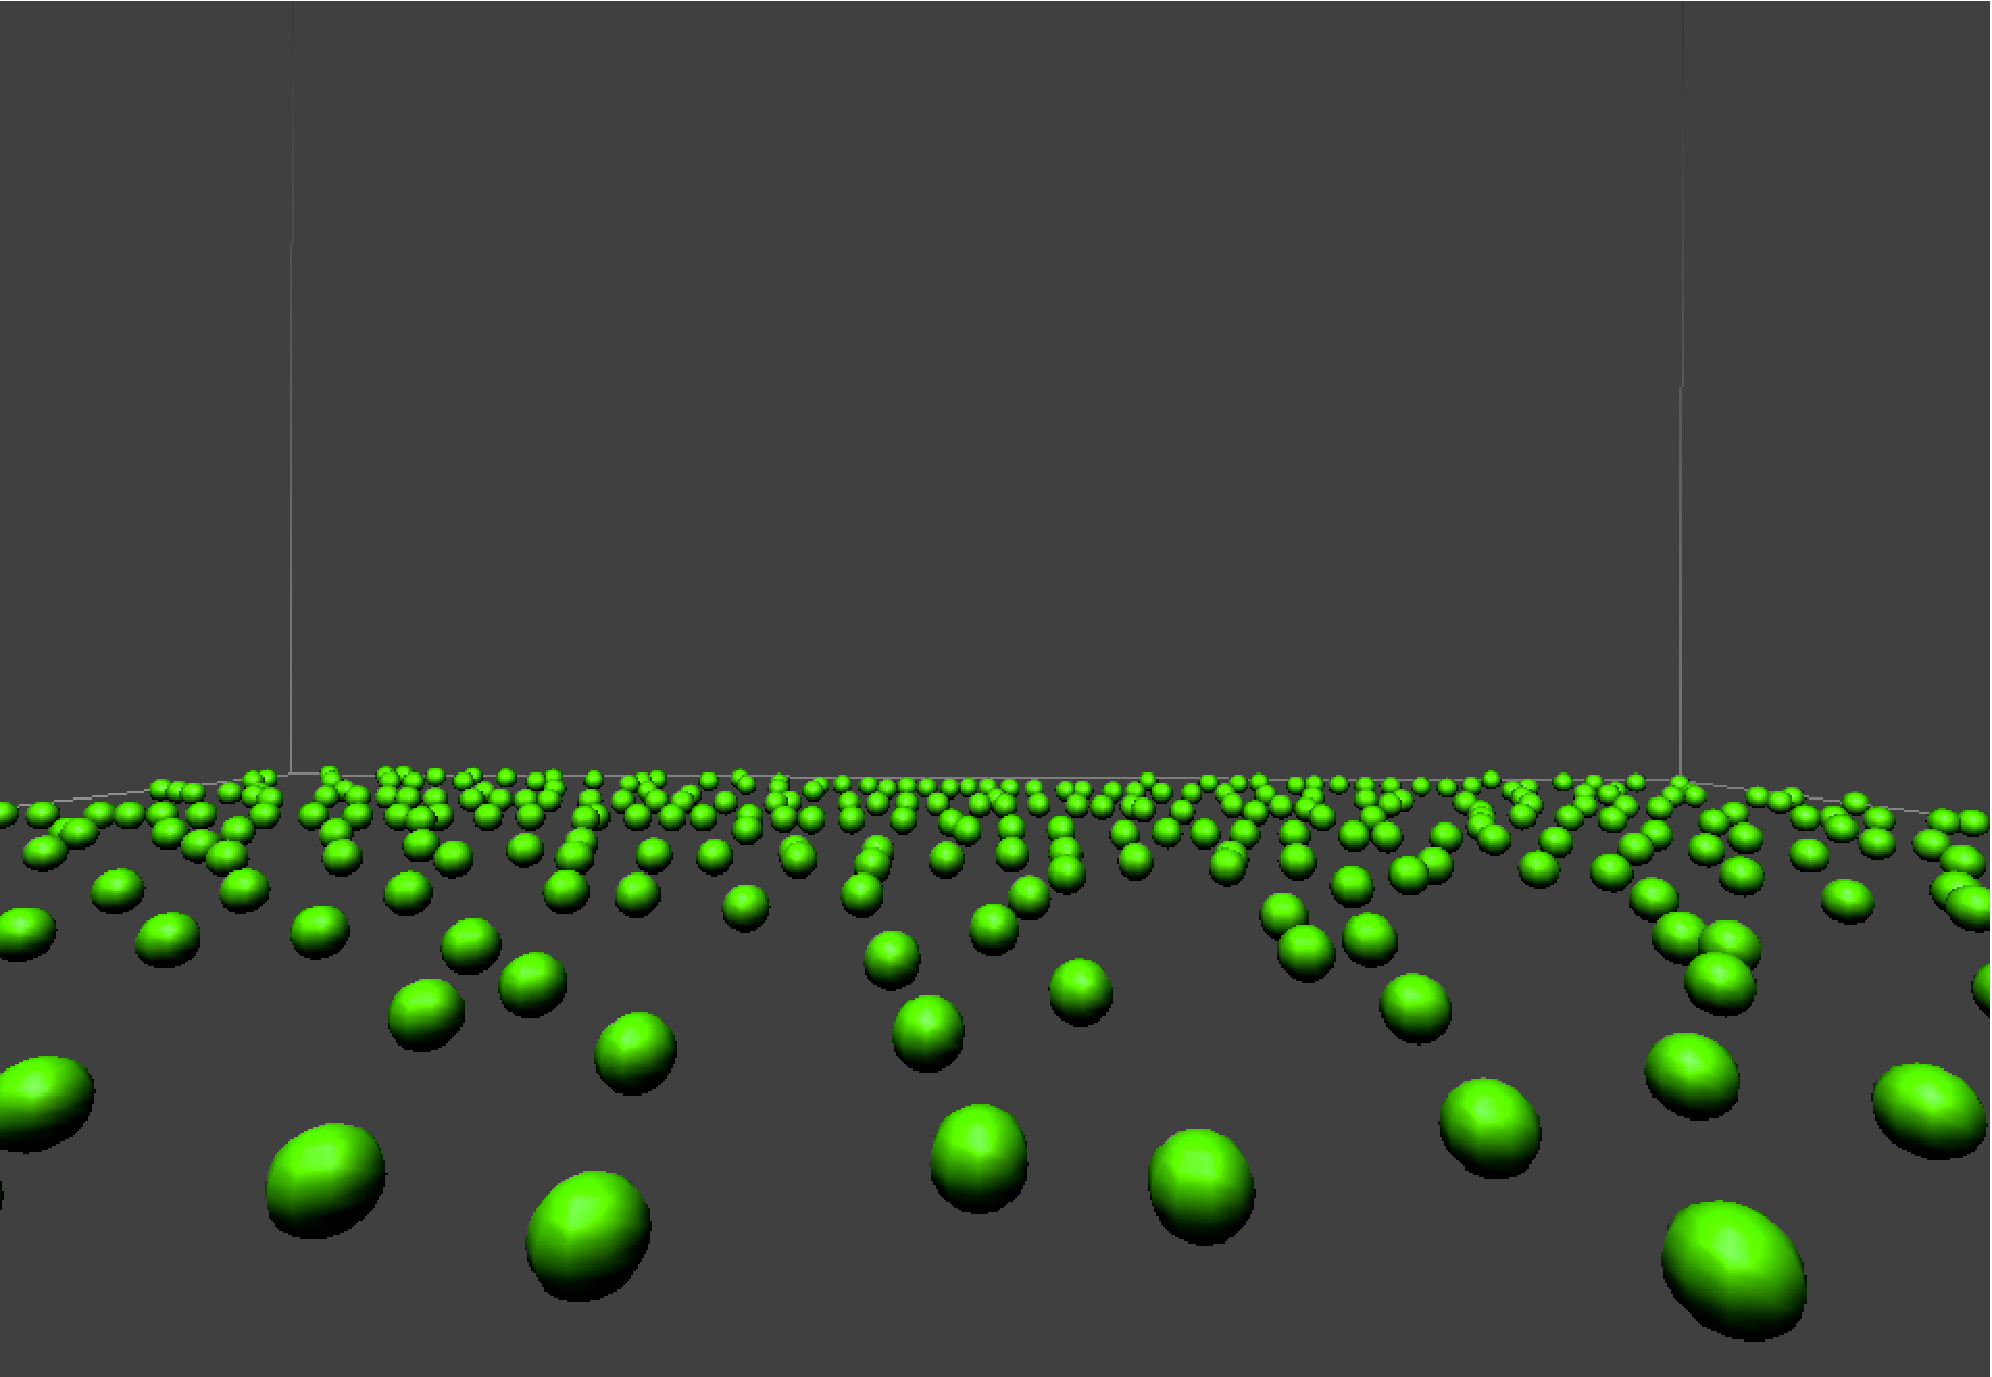
\includegraphics[scale=0.28]{figures/demo_crowds3.pdf}
\end{array}$
\end{center}
\caption{Screenshots of the crowd simulation: showing the initial hose, the boids moving, and the boids already spread through the world.}
\label{crowd_shots}
\end{figure}



